\documentclass[a4paper,10pt,twocolumn]{article}\usepackage[]{graphicx}\usepackage[]{color}
%% maxwidth is the original width if it is less than linewidth
%% otherwise use linewidth (to make sure the graphics do not exceed the margin)
\makeatletter
\def\maxwidth{ %
  \ifdim\Gin@nat@width>\linewidth
    \linewidth
  \else
    \Gin@nat@width
  \fi
}
\makeatother

\definecolor{fgcolor}{rgb}{0.345, 0.345, 0.345}
\newcommand{\hlnum}[1]{\textcolor[rgb]{0.686,0.059,0.569}{#1}}%
\newcommand{\hlstr}[1]{\textcolor[rgb]{0.192,0.494,0.8}{#1}}%
\newcommand{\hlcom}[1]{\textcolor[rgb]{0.678,0.584,0.686}{\textit{#1}}}%
\newcommand{\hlopt}[1]{\textcolor[rgb]{0,0,0}{#1}}%
\newcommand{\hlstd}[1]{\textcolor[rgb]{0.345,0.345,0.345}{#1}}%
\newcommand{\hlkwa}[1]{\textcolor[rgb]{0.161,0.373,0.58}{\textbf{#1}}}%
\newcommand{\hlkwb}[1]{\textcolor[rgb]{0.69,0.353,0.396}{#1}}%
\newcommand{\hlkwc}[1]{\textcolor[rgb]{0.333,0.667,0.333}{#1}}%
\newcommand{\hlkwd}[1]{\textcolor[rgb]{0.737,0.353,0.396}{\textbf{#1}}}%

\usepackage{framed}
\makeatletter
\newenvironment{kframe}{%
 \def\at@end@of@kframe{}%
 \ifinner\ifhmode%
  \def\at@end@of@kframe{\end{minipage}}%
  \begin{minipage}{\columnwidth}%
 \fi\fi%
 \def\FrameCommand##1{\hskip\@totalleftmargin \hskip-\fboxsep
 \colorbox{shadecolor}{##1}\hskip-\fboxsep
     % There is no \\@totalrightmargin, so:
     \hskip-\linewidth \hskip-\@totalleftmargin \hskip\columnwidth}%
 \MakeFramed {\advance\hsize-\width
   \@totalleftmargin\z@ \linewidth\hsize
   \@setminipage}}%
 {\par\unskip\endMakeFramed%
 \at@end@of@kframe}
\makeatother

\definecolor{shadecolor}{rgb}{.97, .97, .97}
\definecolor{messagecolor}{rgb}{0, 0, 0}
\definecolor{warningcolor}{rgb}{1, 0, 1}
\definecolor{errorcolor}{rgb}{1, 0, 0}
\newenvironment{knitrout}{}{} % an empty environment to be redefined in TeX

\usepackage{alltt}

% \usepackage[english,spanish]{babel}
% \usepackage[utf8]{inputenc}
\usepackage{t1enc}
\usepackage{graphicx}
\usepackage{pstricks}
\usepackage{colortab}
\usepackage{pifont}
\usepackage{arydshln}
\usepackage{tipa}
\usepackage{pifont}

\usepackage{icphs2011,multirow,multicol}
\title{Acoustic characteristics of coronal stops in American English and Majorcan Spanish}
\author{Joseph V. Casillas}
\organization{University of Arizona}
\email{jvcasill@email.arizona.edu}
\IfFileExists{upquote.sty}{\usepackage{upquote}}{}
\begin{document}






\twocolumn[
	\begin{@twocolumnfalse}
	\maketitle
	\end{@twocolumnfalse}
	]

\begin{abstract}
    This study explores the acoustic correlates that distinguish coronal stops in American English and Majorcan Spanish. Specifically, we address the differences between Spanish /t/ and English /d/. These phonetically voiceless stops both have short-lag voice-onset time; however, they differ in place of articulation. Spanish /t/ is articulated at dental place, whereas English /d/ is articulated at alveolar place. Mixed effects models explored the spectral moments of the stop bursts and found that, aside from VOT, standard deviation and central moment values differ between the two stops. Binary logistic regression suggests that standard deviation and VOT are the best predictors of place of articulation. 
\end{abstract}

\keywords{VOT, Spanish, English, Spectral moments, Place of articulation}


\section{INTRODUCTION} % (fold)
\label{sec:introduction}

	Previous research has attested that coronal place is the most common for stops in the sound inventories of the world's languages \cite{henton_1992fk}. Spanish and English both have coronal stops /d/ and /t/; however, their phonetic realizations are manifested in different ways. English /d/ and /t/ are produced with an alveolar place of articulation (POA) \cite{picard1987introduction}. Spanish /d/ and /t/, on the other hand, are both produced with a dental POA \cite{hualde2005sounds}. The present investigation set out to explore the acoustic correlates related to place differences amongst these segments.
	
	Aside from the POA, the voicing distinction of the stops in these languages is also realized differently. Specifically, the acoustic correlate voice-onset time (VOT) --the coordination of gestures that results in a difference in time between the onset of phonation and the release of the stop-- is what sets them apart. In English, the voiced stops have short-lag VOT and the voiceless stops have long-lag VOT, whereas in Spanish, the voiced stops have negative, or lead VOT and the voiceless stops have short-lag, positive VOT. A graphical representation of the coronal stops of English and Spanish produced by native speakers can be observed in Figure~\ref{fig:dt_vot}. Note the apparent similarity of Spanish /t/ and English /d/. 

	\begin{figure}[h]
	\centering
	{\scriptsize{\caption{VOT of coronal stops produced by native Spanish speakers (NSP) and native English speakers (NEN).\label{fig:dt_vot}}}}
	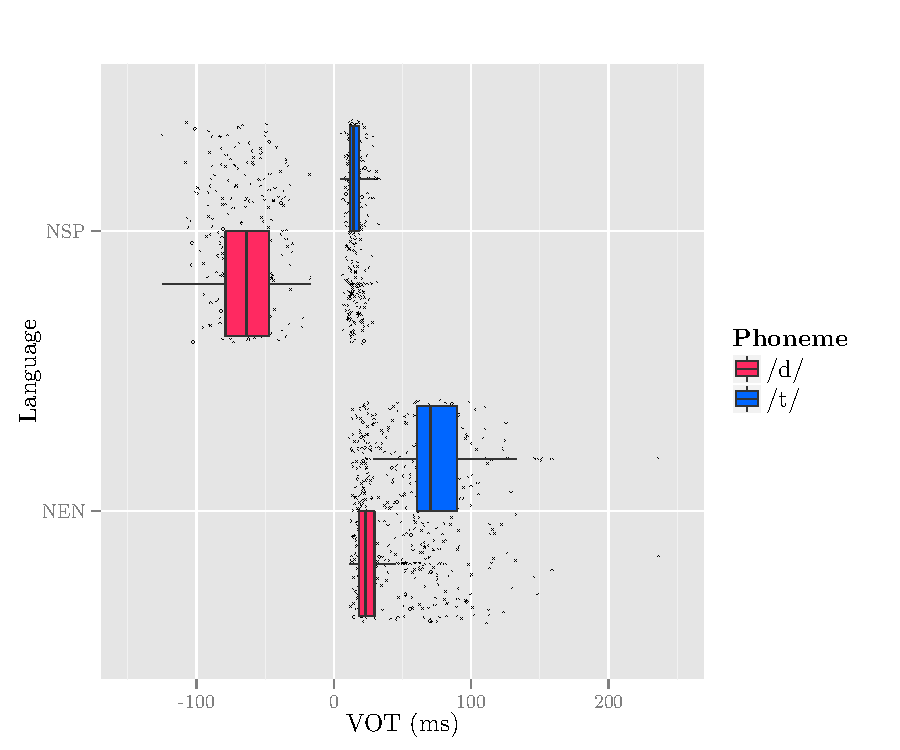
\includegraphics[width=0.435\textwidth]{../figures/vot.pdf}
	\end{figure}


	There is a large body of research that has used VOT to determine the nature of voicing distinctions of stop contrasts in many of the world's languages, but few analyses have used acoustic measures to investigate differences in POA of coronal stops. The fact that both Spanish and English have short-lag, phonetically voiceless stops in their sound inventory (/t/ and /d/, respectively) begs the question as to whether these two segments can be distinguished by any acoustic measures other than VOT. 
	
	The first four spectral moments --center of gravity, standard deviation, skewness, and kurtosis-- provide statistics regarding the shape of a spectrum (i.e. how energy is distributed) \cite{jones2013bloomsbury}. The center of gravity is a measure of the average amplitude of frequency components in the spectrum and is taken as an indication of how high the frequencies are located \cite{Praat}. Standard deviation gives a measure of how far individual frequencies deviate from the center of gravity \cite{jones2013bloomsbury}. The difference between the shape of the spectrum below the center of gravity as compared to the shape above the mean frequency refers to the skewness of the spectrum \cite{Praat}. Kurtosis refers to how far the shape of the spectrum deviates from a Gaussian curve and is taken as an indication of the peakedness of the spectrum relative to the low and high frequencies \cite{hardcastle2012handbook}. 

	Various investigators have used spectral moments to distinguish between place differences in fricatives \cite{gordon2002cross,jongman2000acoustic}; however, \cite{sundara2005acoustic} is the only investigation, to our knowledge, to use spectral moments to analyze place differences in stops. Specifically, she examined coronal stops in Canadian French and Canadian English, which, as is the case with Spanish and English, are realized with dental place and alveolar place, respectively. Her investigation found differences in relative burst intensity, mean frequency, standard deviation, and kurtosis with regard to POA. It remains an open question whether place differences between Spanish /t/ and English /d/ can be accounted for in the same manner. 

% section introduction (end)

\section{METHOD} % (fold)
\label{sec:method}

	The goal of this investigation was to explore the acoustic correlates that differentiate Spanish /t/ from English /d/. Specifically, we measured VOT, the first four spectral moments, and central moment of both short-lag stops in order to see how they were acoustically different. Also of particular interest was the relative importance of each of these measures with regard to place differences of the two phonetically voiceless stops in question. 

	\subsection{Materials} % (fold)
	\label{sub:materials}
	
	In order to address the aforementioned issues, we recorded the speech of twenty-nine participants. Twenty-two were native Spanish speakers (bilinguals in Catalan) between the ages of 18-23 years old, all of which were recruited from the Universitat de les Illes Balears (Majorca, Spain). The native English speakers were undergraduate students at the University of Arizona, recruited from a first-semester Spanish as a second language class. For the purposes of this study, we consider the native English participants to be functionally monolingual. In order to have an equal number of participants in each group, the data from seven of the native Spanish speakers were randomly selected for the present investigation.

	For data collection purposes we devised a list of forty-eight target words, half of which were in English and the other half were in Spanish. The target words contained the voiced and voiceless coronal stops of both languages in word initial position. That is, for each language there was a total of twenty-four words, twelve beginning with /d/ and twelve beginning with /t/. The coronal stops were found in both stressed and unstressed syllables. For each segment except English /t/ there were equal numbers of stressed (6) and unstressed (6) syllables containing the coronal stops. Due to a methodological oversight, the target words for English /t/ contained seven stressed /t/ syllables and five unstressed /t/ syllables. All coronal stops were followed by a low, central or back vowel (/a/ for Spanish and /\ae, \textscripta, \textrhookschwa/ for English). A list of the target words can be found in Table~\ref{words}. 

	\vspace{.1in}
	\begin{table}[ht]
\centering
{\scriptsize{
\begin{tabular}{@{}llll@{}}

\hline \\ [-1.5ex]
\multicolumn{2}{c}{Spanish}       & \multicolumn{2}{c}{English} \\ [1ex]
\hline \\ [-1.5ex]
\emph{da}ba        & \textbf{\emph{t\'ac}til}  & \textbf{\emph{da}gger}    & \emph{ta}bard \\
\emph{da}do        & \textbf{\emph{ta}bla}     & \textbf{\emph{da}mage}    & \emph{ta}bloid \\
\emph{da}ga        & \textbf{\emph{tan}que}    & \textbf{\emph{da}pper}    & \emph{ta}cit \\
\emph{da}ma        & \textbf{\emph{tan}to}     & \textbf{\emph{da}zzle}    & \emph{ta}ckle \\
\emph{da}\~no      & \textbf{\emph{ta}za}      & \textbf{\emph{da}mper}    & \emph{tac}tics \\
\emph{dan}za       & \textbf{\emph{ta}co}      & \textbf{\emph{dan}cing}   & \emph{tan}ker \\
dal\emph{t\'o}nico & \textbf{ta\emph{ber}na}   & \textbf{dan\emph{cette}}  & \emph{tan}trum \\
da\emph{\~nar}     & \textbf{ta\emph{bu}}      & \textbf{dam\emph{na}tion} & ta\emph{boo} \\
da\emph{n\'es}     & \textbf{ta\emph{ma}\~no}  & \textbf{da\emph{ko}ta}    & tambou\emph{rine} \\
da\emph{ne}sa      & \textbf{tam\emph{bi\'en}} & \textbf{dal\emph{to}nian} & ta\emph{pio}ca \\
da\emph{ni}no      & \textbf{tam\emph{po}co}   & \textbf{da\emph{nielle}}  & ta\emph{ttoo} \\
dan\emph{zar}      & \textbf{ta\emph{ba}co}    & \textbf{dan\emph{seur}}   & ta\emph{ttoo}ing \\ [1ex]
\hline
\end{tabular}
}}
\end{table}

	The speakers read all target words in phrase initial position, embedded in the carrier phrase ``X is the word'' or the Spanish equivalent (``X es la palabra''). As this study focused only on words containing coronal stops, all the other words (approx. half the data) were considered distractors. The computer program Praat \cite{Praat} presented the sentences randomly. The English data were recorded in a sound attenuated booth in the Arizona Applied Phonetics Laboratory at the University of Arizona. A Shure SM10A dynamic head-mounted microphone recorded the participants' productions. A Marantz PMD660 pre-amp digitized the signal at 44.1 kHz and 16-bit quantization, and sent the signal to a separate laptop computer where it was recorded in Praat. The same procedure was used in a quiet classroom at the Universitat de les Illes Balears (Majorca, Spain) to record the Spanish productions.

	Each participant provided the dataset with 144 coronal stops (48 target words x 3 repetitions). Thus, a total of 2016 tokens were recorded (48 words x 3 repetitions x 14 participants = 2016 coronal stops); however, for our specific research question, we took a subset of this data (exactly half) containing only Spanish /t/ and English /d/. Five tokens were removed due to mispronunciations or extraneous noise leaving a total of 1003 tokens for statistical analysis. 

	% subsection materials (end)

	\subsection{Measurements} % (fold)
	\label{sub:measurements}
	
	The data were segmented in Praat following standard procedures. Synchronized waveform and spectrographic displays were used to mark the onset of modal voicing and the burst for each of the coronal stops. The onset of voicing was taken to be the first periodic pattern found in the oscillogram \cite{lieberman1988speech}. Next, a Praat script automatically extracted voice-onset time and measures of the shape of the burst spectrum.

	Voice-onset time was calculated as the difference (in ms) between the aforementioned acoustic landmarks (i.e. the onset of modal voicing and the burst). Beginning with the start of the consonantal release, a 30 ms Gaussian window extracted power spectra of the burst. The spectral moments --center of gravity, standard deviation, skew, kurtosis, and the central moment-- were then derived from the extracted spectra. 

	% subsection measurements (end)
% section method (end)

\section{RESULTS} % (fold)
\label{sec:results}

	The present investigation was concerned with the acoustic correlates that differentiate Spanish /t/ from English /d/. To explore this question further, we carried out two main analyses. First, a Linear Mixed Effects model was fit to each acoustic measure detailed above (i.e. VOT, COG, SD, Skew, Kurtosis, and Central moment). In each case the data were best fit with a maximal model. Individual speaker and word items were given random intercepts and language (English /d/ or Spanish /t/) was given random slopes. The likelihood ratio test analyzed statistical significance of language, stress, and a language x stress interaction by assessing the probability of the full model to that of a reduced model based on the chi-squared distribution \cite{winter_2013lr}. We report marginal R$^2$ and conditional R$^2$ as an indication of goodness of fit of the model \cite{Nakagawa2013}. Marginal R$^2$ provides a measure of variance explained without mixed effects and conditional R$^2$ includes them.

	The second analysis explored the extent to which each of the acoustic measures could provide useful information about the place of articulation of the phonetically voiceless phonemes. To this end, we constructed a mixed model using binomial logistic regression with language (Spanish /t/ and English /d/) as the dependent variable, the spectral moments as the predictors, and random intercepts for each speaker. 

	For all analyses, we tested for violations of assumptions of mixed effects models. The tests found that the residuals of center of gravity and central moment were not normally distributed. For this reason we applied a log transformation to each of them so that residual distributions better approached normality in all further tests. Table~\ref{dt_desc} summarizes all measures. 

	% latex table generated in R 3.0.2 by xtable 1.7-1 package
% Sat Nov  9 17:26:23 2013
\begin{table}[t!]
\centering
{\scriptsize{
\begin{tabular}{@{}clcrrccc@{}}
  \hline \\ [-1ex]
\multicolumn{1}{@{}l}{Phon.} & Stress   & VOT   & COG  & \multicolumn{1}{c}{SD} & Skew & Kurt. & CM \\ [1ex]
  \hline \\ [-1ex]
\multirow{2}{*}{/d/}         & Str.     & 23.95 & 6.83 & 1283  & 4.01 & 36.74 & 21.78 \\
                             & Unstr.   & 28.77 & 6.84 & 1202  & 4.74 & 41.65 & 21.70 \\[1ex]
\multirow{2}{*}{/t/}         & Str.     & 14.66 & 6.57 & 624   & 4.77 & 52.13 & 20.61 \\
                             & Unstr.   & 15.90 & 6.55 & 709   & 4.90 & 54.40 & 20.84 \\[1ex]
   \hline
\end{tabular}
}}
\vspace{.05in}
\end{table}


 

	\begin{figure*}[t]
	{\scriptsize{\caption{VOT and spectral moments of Spanish /t/ and English /d/ as a function of stress.\label{fig:all}}}}
	\centering
	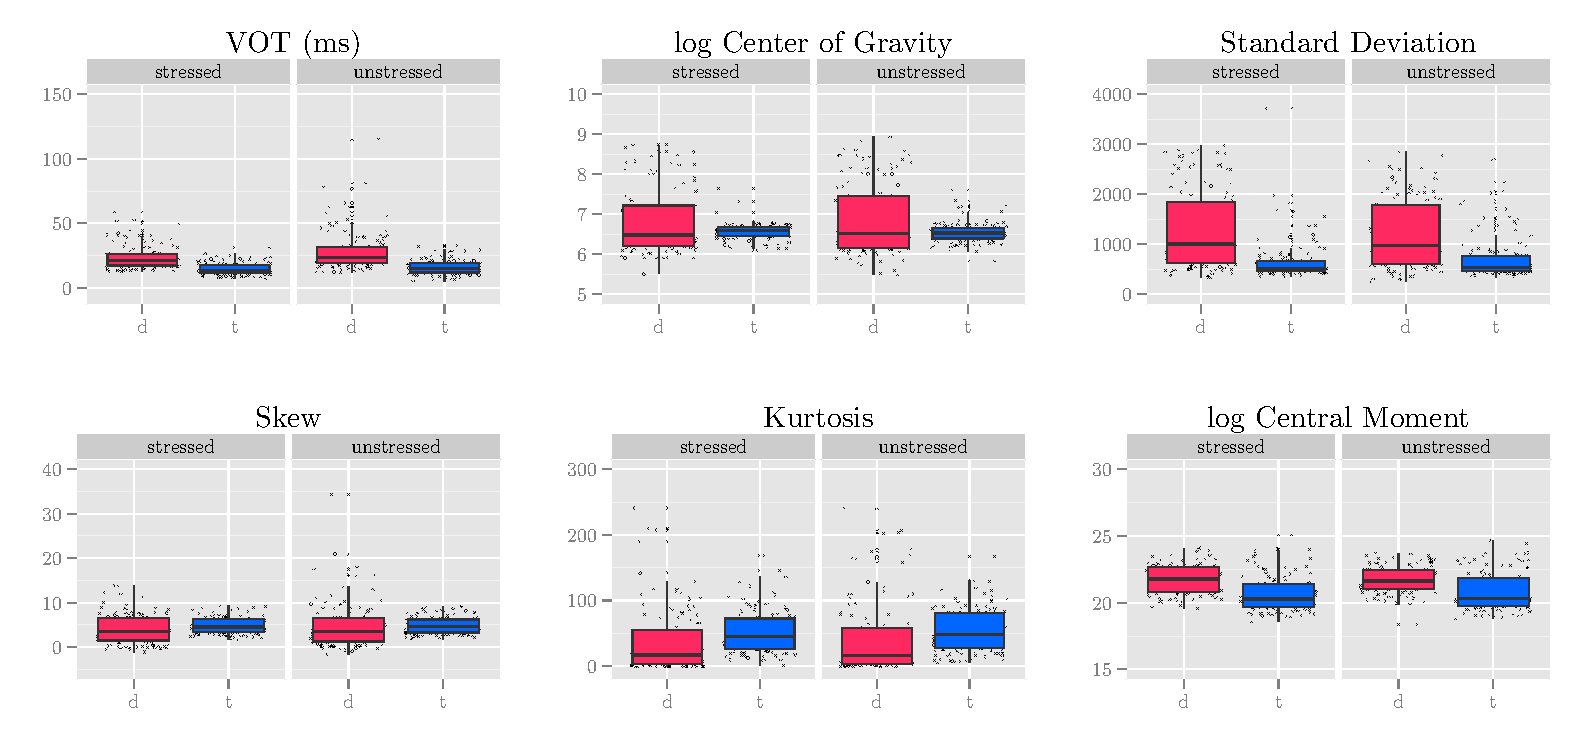
\includegraphics[width=\textwidth]{../figures/dt_all.pdf}
	\end{figure*}

\subsection{Analyses of acoustic measurements} % (fold)
\label{sub:lmem}

	\textbf{Voice-onset time} % (fold)
	\label{par:vot}
	% R2m = 0.12, R2c = 0.76
	The VOT data were analyzed using a linear mixed effects model with VOT as the dependent variable and language and stress as the predictors. Overall the model fit the data well with more variance explained when using a maximal error term (marginal R$^2$ = 0.12; conditional R$^2$ = 0.76). The first graph of Figure~\ref{fig:all} depicts this relationship. One can observe that VOT values differed as a function of language ($\chi$$^2$(1) = 5.43; p < 0.01). Spanish /t/ was shorter than English /d/ by about 11.02 ms $\pm$ 4 (standard errors). There was a small effect for stress ($\chi$$^2$(1) = 5.11; p < 0.03), with shorter VOT values found in stressed segments; however, there was no interaction between language and stress ($\chi$$^2$(1) = 3.11; p > 0.05).
	
	% paragraph vot (end)
	\vspace{.025in}

	\noindent \textbf{Center of gravity} % (fold)
	\label{par:center_of_gravity}
	% R2m = 0.029, R2c = 0.769
	The second graph of Figure~\ref{fig:all} depicts the lack of relationship between center of gravity, language and stress. One can observe clearly that the mean values for English /d/ are much more variable. As before, the center of gravity data were analyzed using a linear mixed effects model with center of gravity as the dependent variable and language and stress as the predictors. Overall the model fit the data well with more variance explained when using a maximal error term (marginal R$^2$ = 0.03; conditional R$^2$ = 0.77). Center of gravity was not affected by language or stress, nor was there an interaction between stress and language (language: $\chi$$^2$(1) = 1.02, p > 0.05; stress: $\chi$$^2$(1) = 0.169, p > 0.05; language by stress: $\chi$$^2$(1) = 0.087, p > 0.05). 

	% paragraph center_of_gravity (end)
	\vspace{.035in}

	\noindent \textbf{Standard Deviation} % (fold)
	\label{par:standard_deviation}
	% R2m = 0.14, R2c = 0.71
	Standard deviation was also analyzed using a linear mixed effects model with standard deviation as the dependent variable and language and stress as the predictors. The model fit the data about as well as the previous models with more variance explained when using a maximal error term (marginal R$^2$ = 0.14; conditional R$^2$ = 0.71). The third graph in Figure~\ref{fig:all} shows that language affected standard deviation ($\chi$$^2$(1) = 4.37; p < 0.05). Spanish /t/ was about 560.10 $\pm$ 230.60 (standard errors) lower than English /d/. That said, stress had no effect on standard deviation nor was there a language by stress interaction (stress: $\chi$$^2$(1) = 0.121, p > 0.05; stress x language: $\chi$$^2$(1) = 2.69, p > 0.05). 

	% paragraph standard_deviation (end)
	\vspace{.025in}

	\noindent \textbf{Skew} % (fold)
	\label{par:skew}
	% R2m = 0.01, R2c = 0.57
	The fourth graph of Figure~\ref{fig:all} shows the data for skew. A model was fit to the data with skew as the dependent variable and language and stress as the predictors. The goodness of fit of the maximal model was acceptable with a conditional R$^2$ of 0.57. The model excluding a maximal error term only explained 1\% of the total variance. The analysis showed no difference between Spanish /t/ and English /d/ with regard to skew ($\chi$$^2$(1) = 0; p > 0.05); however, overall, stress did lower values by about .44 $\pm$ .22 ($\chi$$^2$(1) = 3.93; p < 0.05). Again, there was no interaction between language and stress ($\chi$$^2$(1) = 2.03; p > 0.05). 

	% paragraph skew (end)
	\vspace{.025in}

	\noindent \textbf{Kurtosis} % (fold)
	\label{par:kurtosis}
	% R2m = 0.02, R2c = 0.38
	The same model fit with kurtosis as the dependent variable showed that this measure did not vary as a function of language, stress, nor was there a language by stress interaction (for all models p > 0.05). The fifth graph in Figure~\ref{fig:all} provides a visual representation of the data. Overall, the model explained less of the variance in comparison to the previous models (marginal R$^2$ = 0.02; conditional R$^2$ = 0.38).

	% paragraph kurtosis (end)
	\vspace{.025in}

	\noindent \textbf{Central moment} % (fold)
	\label{par:central_moment}
	% R2m = 0.216, R2c = 0.430
	Finally, the central moment data was fit to the same model as the previous acoustic measures. The model accounted for less than half the the variance (marginal R$^2$ = 0.22; conditional R$^2$ = 0.43). The final boxplot of Figure~\ref{fig:all} shows the relationship between central moment values for each of the segments. The model showed that language affected central moment ($\chi$$^2$(1) = 4.38, p < 0.05), by lowering Spanish /t/ by about 1.24 hz $\pm$ .46 (standard errors). Stress did not affect central moment values ($\chi$$^2$(1) = 0.014, p > 0.05), nor was there a language by stress interaction ($\chi$$^2$(1) = 4.28, p > 0.05).
	% paragraph central_moment (end)

% subsection lmem (end)

\subsection{Weight of spectral moment effects} % (fold)
\label{sub:hierarchical_model}

	The second analysis explored the extent to which each of the acoustic measures could provide useful information about the place of articulation of the phonetically voiceless phonemes. To this end, we constructed a mixed model using binomial logistic regression with language (Spanish /t/ and English /d/) as the dependent variable, the spectral moments as the predictors, and random intercepts for each speaker.\footnote{{\scriptsize{One of the assumptions of this type of model is that the predictors cannot be intercorrelated. If, for example, predictor X and predictor Y were correlated, the relationship was orthogonalized by taking the residuals of a linear model in which X predicted Y and using them as the predictor in the main binomial regression.}}} The purpose of this analysis was to determine which of the acoustic correlates added most to the fit of the model. Table~\ref{model_sum} summarizes the results. Standard deviation was presumably the best acoustic correlate as it improved the fit of the model by explaining 26.4\% of the variance. The next best measure was VOT, explaining an additional 11.3\% of the variance. Interestingly, the model optimally predicted the identity of the two stops when kurtosis and central moment were removed (68\% of total variance explained).

	\vspace{.1in}
	\begin{table}[ht]
\centering
\caption{Regression analysis of /d/-/t/.\label{model_sum}}
\begin{tabular}{@{}lccrr@{}}

\hline \\ [-1ex]
Metric & \emph{R}$^2$ & \emph{R}$^2_{\ change}$ & \emph{F}$_{change}$ & \emph{p-value} \\ [1ex]
\hline \\ [-1ex]
SD  & .353  & .353 & 175.39 & < 0.001 \\
COG & .376  & .023 &  14.01 & < 0.001 \\
RI  & .425  & .049 &  30.01 & < 0.001 \\
Sk  & .426  & .001 &   0.08 & > 0.05  \\
Kt  & .432  & .006 &   4.36 & < 0.04  \\
\hline
\end{tabular}
\vspace{.05in}
\end{table}

% #         R2  R2 change      F       P 
% # sd  = .353       .353 175.39 < 0.001
% # cog = .376       .023  14.01 < 0.001
% # ri  = .425       .049  30.01 < 0.001
% # sk  = .426       .001   0.08 > 0.05 
% # kt  = .432       .006   4.36 < 0.04 

	\vspace{.05in}
% subsection hierarchical_model (end)
% section results (end)



\section{DISCUSSION} % (fold)
\label{sec:discussion}

	The results of the two analyses showed that the phonetically voiceless coronal stops of English and Spanish can be distinguished by VOT and the spectral shape of the stop burst. Importantly, the present study indicates that the place of articulation differences found in Spanish /t/ and English /d/ can be accounted for using measures of standard deviation and central moment. Center of gravity, skew, and kurtosis appeared to be unaffected by the place of articulation of the stops in our data. 

	Our results partially corroborate the findings of \cite{sundara2005acoustic}, who investigated coronal stops in Canadian English and Canadian French. The stop contrasts in these two languages resemble those of English and Spanish in that there are two phonetically voiceless stops that are distinguished principally on place differences (alveolar English /d/ and dental French /t/, as is the case in the present study). In their data, values of standard deviation also varied across the two stops; however, they also encountered significant differences for kurtosis. Our study did not find any significant differences based on kurtosis, but it was shown to add positively to the fit of the logistic regression, accounting for approximately \%10 more variance explained. 

	The present study contributes language-specific acoustic characteristics of bursts in the short-lag coronal stops of American English and Majorcan Spanish. The findings provide the groundwork for future studies on bilinguals and L2 learners of either language. Future research should explore other measures --such as relative burst intensity, which was found to vary cross-linguistically in \cite{sundara2005acoustic}-- to advance our knowledge of stops in Spanish and English. 

% section discussion (end)

\newpage
\bibliographystyle{abbrv} 
\bibliography{vot.bib}
\vspace{-.15in}
\theendnotes

\end{document}

